\documentclass[noauthor,nooutcomes,hints,handout]{ximera}

\graphicspath{  
{./}
{./whoAreYou/}
{./drawingWithTheTurtle/}
{./bisectionMethod/}
{./circles/}
{./anglesAndRightTriangles/}
{./lawOfSines/}
{./lawOfCosines/}
{./plotter/}
{./staircases/}
{./pitch/}
{./qualityControl/}
{./symmetry/}
{./nGonBlock/}
}


%% page layout
\usepackage[cm,headings]{fullpage}
\raggedright
\setlength\headheight{13.6pt}


%% fonts
\usepackage{euler}

\usepackage{FiraMono}
\renewcommand\familydefault{\ttdefault} 
\usepackage[defaultmathsizes]{mathastext}
\usepackage[htt]{hyphenat}

\usepackage[T1]{fontenc}
\usepackage[scaled=1]{FiraSans}

%\usepackage{wedn}
\usepackage{pbsi} %% Answer font


\usepackage{cancel} %% strike through in pitch/pitch.tex


%% \usepackage{ulem} %% 
%% \renewcommand{\ULthickness}{2pt}% changes underline thickness

\tikzset{>=stealth}

\usepackage{adjustbox}

\setcounter{titlenumber}{-1}

%% journal style
\makeatletter
\newcommand\journalstyle{%
  \def\activitystyle{activity-chapter}
  \def\maketitle{%
    \addtocounter{titlenumber}{1}%
                {\flushleft\small\sffamily\bfseries\@pretitle\par\vspace{-1.5em}}%
                {\flushleft\LARGE\sffamily\bfseries\thetitlenumber\hspace{1em}\@title \par }%
                {\vskip .6em\noindent\textit\theabstract\setcounter{question}{0}\setcounter{sectiontitlenumber}{0}}%
                    \par\vspace{2em}
                    \phantomsection\addcontentsline{toc}{section}{\thetitlenumber\hspace{1em}\textbf{\@title}}%
                     }}
\makeatother



%% thm like environments
\let\question\relax
\let\endquestion\relax

\newtheoremstyle{QuestionStyle}{\topsep}{\topsep}%%% space between body and thm
		{}                      %%% Thm body font
		{}                              %%% Indent amount (empty = no indent)
		{\bfseries}            %%% Thm head font
		{)}                              %%% Punctuation after thm head
		{ }                           %%% Space after thm head
		{\thmnumber{#2}\thmnote{ \bfseries(#3)}}%%% Thm head spec
\theoremstyle{QuestionStyle}
\newtheorem{question}{}



\let\freeResponse\relax
\let\endfreeResponse\relax

%% \newtheoremstyle{ResponseStyle}{\topsep}{\topsep}%%% space between body and thm
%% 		{\wedn\bfseries}                      %%% Thm body font
%% 		{}                              %%% Indent amount (empty = no indent)
%% 		{\wedn\bfseries}            %%% Thm head font
%% 		{}                              %%% Punctuation after thm head
%% 		{3ex}                           %%% Space after thm head
%% 		{\underline{\underline{\thmname{#1}}}}%%% Thm head spec
%% \theoremstyle{ResponseStyle}

\usepackage[tikz]{mdframed}
\mdfdefinestyle{ResponseStyle}{leftmargin=1cm,linecolor=black,roundcorner=5pt,
, font=\bsifamily,}%font=\wedn\bfseries\upshape,}


\ifhandout
\NewEnviron{freeResponse}{}
\else
%\newtheorem{freeResponse}{Response:}
\newenvironment{freeResponse}{\begin{mdframed}[style=ResponseStyle]}{\end{mdframed}}
\fi



%% attempting to automate outcomes.

%% \newwrite\outcomefile
%%   \immediate\openout\outcomefile=\jobname.oc
%% \renewcommand{\outcome}[1]{\edef\theoutcomes{\theoutcomes #1~}%
%% \immediate\write\outcomefile{\unexpanded{\outcome}{#1}}}

%% \newcommand{\outcomelist}{\begin{itemize}\theoutcomes\end{itemize}}

%% \NewEnviron{listOutcomes}{\small\sffamily
%% After answering the following questions, students should be able to:
%% \begin{itemize}
%% \BODY
%% \end{itemize}
%% }
\usepackage[tikz]{mdframed}
\mdfdefinestyle{OutcomeStyle}{leftmargin=2cm,rightmargin=2cm,linecolor=black,roundcorner=5pt,
, font=\small\sffamily,}%font=\wedn\bfseries\upshape,}
\newenvironment{listOutcomes}{\begin{mdframed}[style=OutcomeStyle]After answering the following questions, students should be able to:\begin{itemize}}{\end{itemize}\end{mdframed}}



%% my commands

\newcommand{\snap}{{\bfseries\itshape\textsf{Snap!}}}
\newcommand{\flavor}{\link[\snap]{https://snap.berkeley.edu/}}
\newcommand{\mooculus}{\textsf{\textbf{MOOC}\textnormal{\textsf{ULUS}}}}


\usepackage{tkz-euclide}
\tikzstyle geometryDiagrams=[rounded corners=.5pt,ultra thick,color=black]
\colorlet{penColor}{black} % Color of a curve in a plot



\ifhandout\newcommand{\mynewpage}{\newpage}\else\newcommand{\mynewpage}{}\fi


\title{Symmetries of the regular hexagon}
\author{Bart Snapp}

\begin{document}
\begin{abstract}
  We explore the symmetries of the regular hexagon.
\end{abstract}
\maketitle

\begin{listOutcomes}
\item Describe symmetries of the regular hexagon without finding them
  all via pictures.
\item Think of the symmetries of the regular hexagon as functions.
\item Use \snap\ to compose symmetries.
\item Use the algebra of symmetries to understand a composition of
  symmetries.
\end{listOutcomes}
\mynewpage


\begin{question}
  The symmetries of the regular hexagon are those that leave it
  unchanged. Let $e$ be the do-nothing symmetry, $r$ be a clockwise
  $60^\circ$ rotation about the center of the hexagon, and $f$ be a
  flip across a vertical line down the middle of the hexagon.

  
  How many symmetries are there of the regular hexagon? Just
  EXPLAIN with words and AS FEW PICTURES AS NECESSARY.
  \begin{freeResponse}
    To start, there's the do-nothing symmetry, $e$. Then there are
    $5$ clockwise rotations, $r$, $r^2$, $r^3$, $r^4$, and $r^5$.

    There are flips across a line perpendicular to every face of the
    hexagon. There are $3$ of these.

    There are flips across lines through opposite vertices. There are
    $3$ of these.

    Hence there are $12$ symmetries of the regular hexagon.
  \end{freeResponse}
\end{question}
\mynewpage

\begin{question}
  Let $e$ be the do-nothing symmetry, $r$ be a clockwise $60^\circ$
  rotation about the center of the hexagon, and $f$ be a flip across a
  vertical line down the middle of the hexagon.  When $e$ is applied,
  the hexagon looks like this:
  \[
  \raisebox{-.4\height}{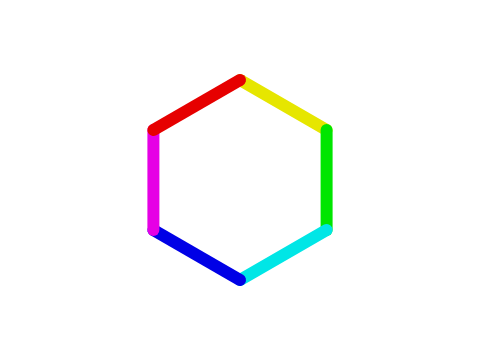
\includegraphics[width=2.5in]{eHex.png}}\resizebox{.7in}{!}{$\overset{\scriptscriptstyle e}{\mapsto}$} \raisebox{-.4\height}{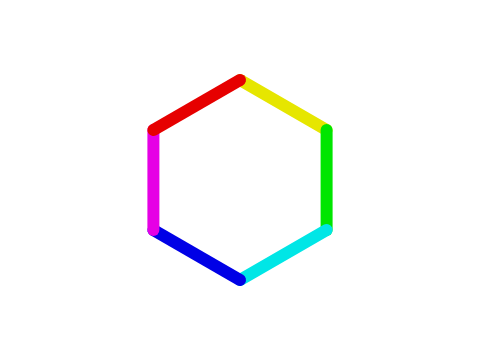
\includegraphics[width=2.5in]{eHex.png}}
  \]
  Display the result of applying the following functions
  (actions/transformations) to your hexagon:
  \begin{enumerate}
  \item $fr$
  \item $fr^4$
  \item $r^3 f$
  \item $f r^3$
  \end{enumerate}
  In each case, show off your work by displaying your STAGE.  
  \begin{freeResponse}
    \begin{enumerate}
    \item For $fr$ I have
      \[
      \raisebox{-.4\height}{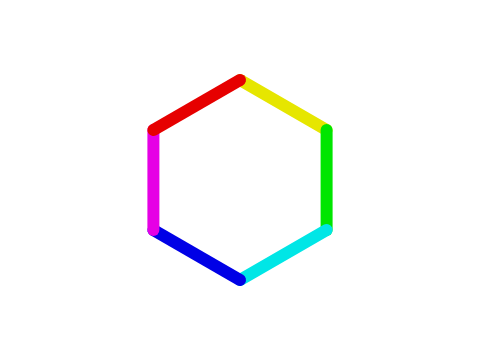
\includegraphics[width=2.5in]{eHex.png}}\resizebox{.7in}{!}{$\overset{\scriptscriptstyle fr}{\mapsto}$} \raisebox{-.4\height}{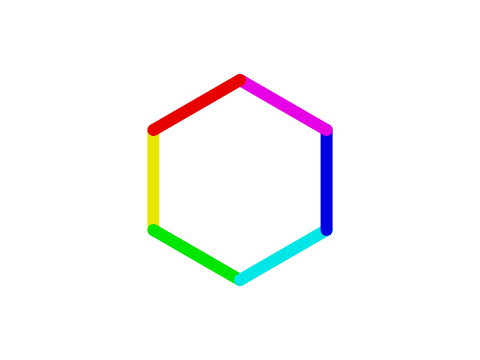
\includegraphics[width=2.5in]{r5fHex.png}}
      \]
    \item For $fr^4$ I have
      \[
      \raisebox{-.4\height}{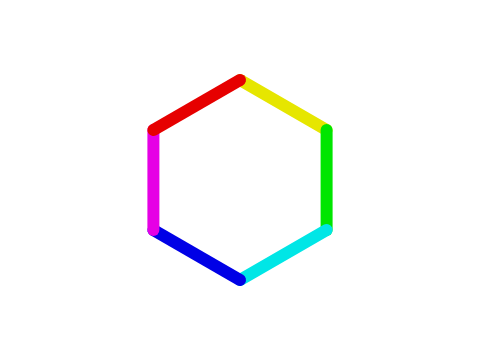
\includegraphics[width=2.5in]{eHex.png}}\resizebox{.7in}{!}{$\overset{\scriptscriptstyle fr^4}{\mapsto}$} \raisebox{-.4\height}{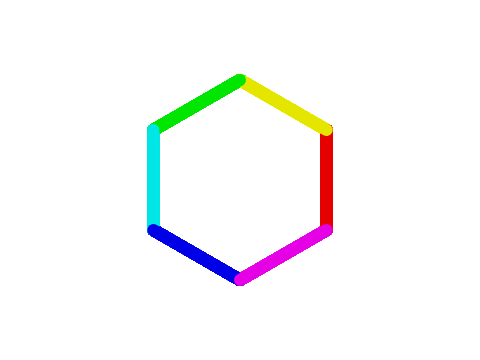
\includegraphics[width=2.5in]{r2fHex.png}}
      \]
    \item For $r^3f$ I have
      \[
      \raisebox{-.4\height}{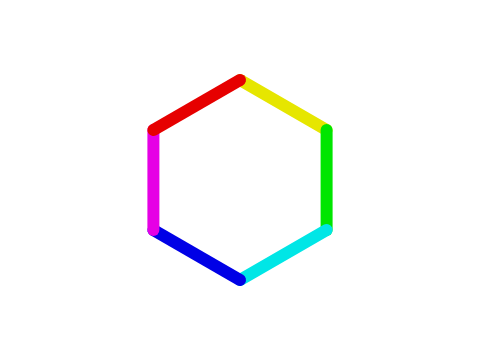
\includegraphics[width=2.5in]{eHex.png}}\resizebox{.7in}{!}{$\overset{\scriptscriptstyle  r^3f}{\mapsto}$} \raisebox{-.4\height}{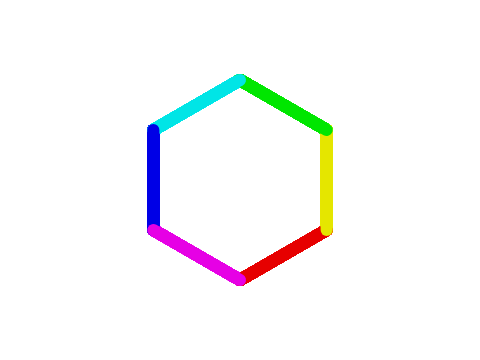
\includegraphics[width=2.5in]{r3fHex.png}}
      \]
    \item For $fr^3$ I have
      \[
      \raisebox{-.4\height}{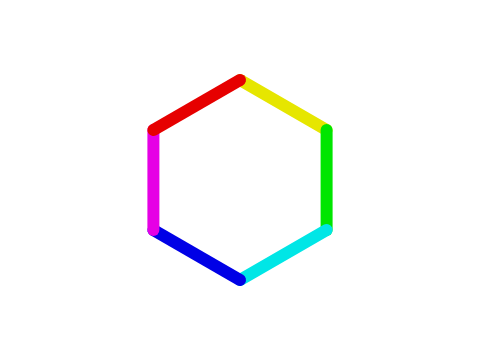
\includegraphics[width=2.5in]{eHex.png}}\resizebox{.7in}{!}{$\overset{\scriptscriptstyle fr^3}{\mapsto}$} \raisebox{-.4\height}{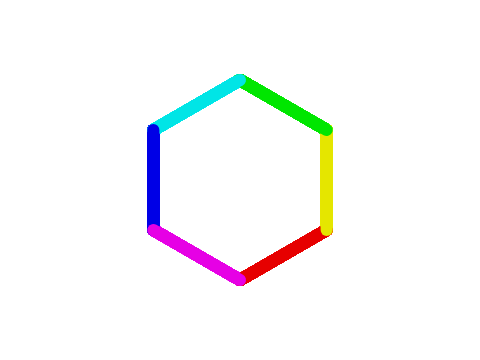
\includegraphics[width=2.5in]{r3fHex.png}}
      \]
    \end{enumerate}
    \end{freeResponse}
\end{question}
\mynewpage


\begin{question}
 EXPRESS each of the symmetries below as one of:
 \[
 e,r,r^2,r^3,r^4,r^5,f,rf,r^2f,r^3f, r^4f,r^5f.
 \]

 \begin{enumerate}
 \item $fr$
 \item $fr^2$
 \item $fr^3$
 \item $fr^4$
 \item $fr^5$
 \item $fr^7f^2r^9f^5r^4f^3$
 \end{enumerate}
 \begin{freeResponse}
   \begin{enumerate}
   \item $fr = r^5f$
   \item $fr^2 = r^4f$
   \item $fr^3 = r^3f$
   \item $fr^4 = r^2f$
   \item $fr^5 = rf$
   \item And finally,
     \begin{align*}
    f^3r^5f^7r^9 &= fr^5fr^3\\
    &= rf^2r^3\\
    &= r^4.
     \end{align*}
   \end{enumerate}
 \end{freeResponse}
\end{question}
\end{document}
